\documentclass[11pt]{article}
\usepackage[margin=1.9cm]{geometry}
\usepackage{graphicx}
\usepackage{booktabs}
\usepackage{amsmath}
\usepackage{hyperref}
\usepackage{titlesec}
\usepackage{enumitem}
\usepackage{parskip}
\setlength{\parskip}{0.3em plus 0.1em minus 0.1em}
\usepackage{xcolor}

\titleformat{\section}{\large\bfseries}{\thesection}{0.6em}{}
\titleformat{\subsection}{\normalsize\bfseries}{\thesubsection}{0.6em}{}
\titlespacing*{\section}{0pt}{1.1em}{0.5em}
\titlespacing*{\subsection}{0pt}{0.9em}{0.4em}

\hypersetup{colorlinks=true, linkcolor=blue, urlcolor=blue}
\raggedbottom
\setlength{\textfloatsep}{8pt plus 1pt minus 1pt}
\setlength{\intextsep}{6pt plus 1pt minus 1pt}
\setlength{\floatsep}{6pt plus 1pt minus 1pt}

\title{\vspace{-1.5em}\textbf{JP's Portfolio}}
\author{Jyoti Pandey \quad Keshav Kumar}
\date{}

\begin{document}
\maketitle
\vspace{-3em}

\section{Problem and Strategy Overview}

Each team constructs and manages a maximum 10-stock equity portfolio drawn from
the Nifty 100, Nifty Midcap 100 and Nifty Smallcap 100 universes, backtested from 1 January 2021
to 31 December 2025 with a virtual corpus of Rs 1 crore. The primary ranking metric is Total Net
PnL, and a forward-looking out-of-sample stress test on 1 January 2026 to 30 June 2026 checks that the
strategy generalises beyond the backtest window.

The central idea is a single, fully systematic composite-factor strategy applied identically to
every eligible stock: a quarterly-rebalanced ranking on three price-based factors (12-1 month
momentum, low-volatility, and a trend-quality measure), sized by inverse volatility with a
concentration cap on the initial selection, with any leftover cash redeployed into the names
already selected. The design was deliberately kept simple and fully rule-based, so it can be
traced exactly how the portfolio was produced at any point in time. It was also validated using a
train/test split and a rolling-window robustness check, rather than chosen purely for the highest
in-sample return, in anticipation of the forward stress test.

\section{Data}

\textbf{Universe.} The eligible universe ($\approx$300 stocks) was built by combining the
current NSE constituent lists for Nifty 100, Nifty Midcap 100 and Nifty Smallcap 100. A handful
of symbols appear on more than one list; these are de-duplicated to a single entry recording
every index the stock belongs to. Since point-in-time historical index membership is not freely
available, the current constituent lists are applied retroactively across the full 2021--2025
backtest; this is a stated simplification (see Limitations).

\textbf{Prices.} Daily OHLCV data for every universe stock and for the two benchmark indices was
downloaded via the \texttt{yfinance} package, covering well before the 2021 backtest start
through the end of the backtest. Prices are auto-adjusted closes (dividend- and split-adjusted).
Only the adjusted \emph{close} column feeds the model itself; open/high/low/volume are downloaded
but not used by the current strategy. The extra pre-2021 history is a buffer so the 252-day
momentum/quality lookback has sufficient data from day one of the backtest. At each quarterly
rebalance, any stock with less than 95\% price coverage over the lookback window (mostly recent
IPOs) is excluded from that quarter's ranking rather than treated as having a zero or missing
score.

\textbf{Fundamental data.} No fundamental data (earnings, book value, ROE, etc.) is used. This
is a deliberate choice, not an oversight: reliable, point-in-time fundamental data free of
look-ahead bias is not readily available for 300 stocks spanning large, mid and small caps in
India. Building the model on price data alone also keeps the same formula applicable to every
stock without exception.

\section{Methodology}

\subsection{Stock selection}
Every quarter (first trading day of Jan/Apr/Jul/Oct), a composite score is computed for every
eligible stock:
\[
\text{Composite} = 0.5\times\big[0.5\,Z(\text{Momentum}) + 0.5\,Z(\text{Low-Vol})\big] + 0.5\,Z(\text{Quality})
\]
where:
\begin{itemize}[leftmargin=1.2em, itemsep=1pt, topsep=0.2em]
\item \textbf{Momentum} is the 12-month price return skipping the most recent month (the
standard ``12-1'' construction, which avoids short-term reversal effects).
\item \textbf{Low-Vol} is the negative of the trailing 90-day daily return standard deviation.
\item \textbf{Quality} is the $R^2$ of a linear trend fit to log-price over the same 12-month
window, which penalises spiky, parabolic price paths in favour of smoothly-trending ones.
\end{itemize}
Each factor is cross-sectionally
z-scored across all stocks with at least 95\% price history over the lookback window; stocks
without enough history (mostly recent IPOs) are automatically excluded that quarter. The 10
highest composite-score stocks are then selected. Section 3.3 works through this scoring for one
real stock and rebalance date.

\textbf{Why these three factors.} Momentum and low-volatility are two of the most extensively
documented factors in equity research, and they are deliberately complementary rather than
redundant. Momentum drives the return by following stocks that are already trending, while
low-volatility manages risk, since momentum alone is known to be prone to sharp reversals (a
``momentum crash'') after a strong run. The quality/trend-smoothness factor was added for a
specific, tested reason rather than assumed upfront. An earlier two-factor version of this
strategy underperformed the benchmark in a blind 2025 test (Section 7), and the cause was
concentration in momentum names with erratic rather than steady price paths--exactly the names
most prone to reversal. Adding trend-quality was confirmed, not merely assumed, to fix that
weakness (Section 7). Value and fundamental-quality factors were excluded for the
data-reliability reason above. Size is already handled structurally by the universe spanning
three cap segments. Liquidity was not added separately since it overlaps heavily with
volatility. And a short-term reversal factor was rejected because it would work against momentum
over a similar horizon.

\subsection{Weighting}
Selected stocks are sized inverse to their own trailing 90-day volatility (the same volatility
used in the Low-Vol factor), so that size is set by each stock's own risk rather than by how
high it ranks on the noisier composite score. Raw inverse-volatility affinities are shifted down
by their minimum (plus a small constant) before normalising, then capped at 15\% of portfolio
value per name. Any excess above the cap is redistributed proportionally among the remaining
names, iterated until no name exceeds the cap. This keeps a single very low-volatility name
from dominating the book. Section 3.3 continues the worked example with this stock's weight
assignment.

The 15\% cap governs this initial selection and sizing pass only. Because the ten target weights
sum to exactly 100\% while every buy also carries the 0.1\% transaction cost on top, fully funding
all ten names would need slightly more than the available capital; the lowest-priority name is
typically left short once whole-share flooring is applied (Section 7). Rather than let that
shortfall sit idle as cash, it is redeployed into the names that were funded, proportional to
their own target weights -- a more concentrated bet on names already selected, rather than
forcing capital into the unfunded (typically highest-volatility) name or leaving it unused. This
redeployment pass is deliberately allowed to push a name above 15\%: the cap is a selection-risk
control, not a hard ceiling on what happens to leftover cash from an already-capped selection.
This design was chosen over leaving the shortfall as cash and over a version of redeployment that
re-enforces the 15\% cap during top-up, after testing all three: it won on CAGR, Sharpe and the
2025 held-out test, and matched or led on the 20-quarter rolling hit-rate.

\subsection{Worked example}
At the 1 October 2025 rebalance, across that day's $\approx$277 eligible stocks, 12-1 month
momentum had cross-sectional mean $-2.55\%$ and standard deviation $26.06\%$. BHARTIARTL's own
momentum was $+7.45\%$, giving $Z(\text{Momentum}) = (7.45 - (-2.55))/26.06 = 0.38$. The same
$Z=(x-\text{mean})/\text{s.d.}$ formula applied to its trailing 90-day volatility (Low-Vol
$-1.03\%$ vs. a cross-sectional mean of $-1.75\%$, s.d. $0.61\%$) gives $Z(\text{Low-Vol})=1.18$,
and applied to its trend-quality $R^2$ ($0.76$ vs. a mean of $0.32$, s.d. $0.25$) gives
$Z(\text{Quality})=1.75$. Its composite score, $0.5\times[0.5(0.38)+0.5(1.18)]+0.5(1.75)=1.27$,
ranked 9th overall, placing it in the top 10 selected that quarter (Table 2).

For weighting, BHARTIARTL's trailing 90-day volatility was $1.03\%$, giving a raw
inverse-volatility affinity of $1/0.0103=97.0$. Across the ten selected names that quarter, the
lowest affinity (Force Motors) was $26.3$; shifting every affinity down by this minimum plus a
small constant ($\epsilon=0.1$) gives BHARTIARTL a shifted affinity of $97.0-26.3+0.1=70.8$,
which is $70.8/345.6=20.5\%$ of the shifted total across all ten names. Since this exceeds the
15\% cap, BHARTIARTL is capped at exactly $15\%$, and the excess $5.5$ percentage points is
redistributed proportionally among the other nine names.

\subsection{Rebalancing and risk management}
Stock selection and target weights are decided quarterly (first trading day of
Jan/Apr/Jul/Oct); positions are held unchanged between rebalances. Only the delta needed to
reach the new target is traded for names that remain selected, while dropped names are fully
sold and new entrants are bought to target. A selected stock already trading below its own
200-day average on the rebalance date itself is not bought that quarter -- a one-time check at
the point of purchase, not ongoing daily monitoring (Section 7). A flat 0.1\% transaction cost is
charged on the notional value of every executed buy and sell, deducted directly from cash, so it
compounds into every subsequent decision rather than being a cosmetic adjustment applied at the
end.

\subsection{Consistency and parameter selection}
The same formula, thresholds and rules are applied to every one of the $\approx$300
eligible stocks with no per-stock discretion. The one free parameter with any real tuning
behind it--the 50\% weight given to the quality factor--was selected using only 2021--2024
training data and full-backtest metrics, deliberately excluding the 2025 held-out test, via a
0.001-resolution grid search. That search confirmed the chosen weight sits inside a genuine
stable plateau (0.499 and 0.500 are bit-identical on the full backtest; 0.501--0.503 sit within
0.1 percentage point of the same result) rather than an isolated, fragile spike. This distinction
matters because it is easy to overfit a single free parameter to one backtest window.

\subsection{Key assumptions}
\begin{itemize}[leftmargin=1.2em, itemsep=1pt, topsep=0.2em]
\item Trades execute at the same-day closing price as the signal date (standard close-to-close convention).
\item All trades are in whole shares (no fractional shares), with target rupee allocations floored to the nearest full share.
\item Idle or exited cash earns 0\%.
\item Corporate actions are handled via Yahoo Finance's auto-adjusted close series.
\item No slippage, shorting or leverage is modelled beyond the stated 0.1\% transaction cost.
\end{itemize}

\section{Tools and Software Used}
The entire pipeline is written in Python 3, using \texttt{pandas} and \texttt{numpy} for data
handling and the day-by-day backtest simulation, and \texttt{yfinance} for price data
acquisition. No machine-learning or numerical-optimisation library is used: the model is a
transparent, rules-based factor score rather than a fitted or black-box one. This was a
deliberate choice, given the requirement that another evaluator be able to understand exactly
how the portfolio was produced. \texttt{matplotlib} was used for the chart in this report, and the
report itself is typeset in \LaTeX{}. The complete code is in the accompanying GitHub
repository (see the README for how to reproduce every number in this report).

\section{Results and Performance Metrics}

\begin{table}[h]
\centering
\begin{tabular}{lr}
\toprule
\textbf{Metric} & \textbf{Value} \\
\midrule
Final Portfolio Value & Rs 7.37 crore \\
Total Net PnL & Rs 6.37 crore \\
Absolute Return & 637.19\% \\
Annualised Return (CAGR) & 49.15\% \\
Maximum Drawdown & $-$30.07\% \\
Sharpe Ratio (rf = 0\%) & 2.35 \\
Gain-to-Loss Ratio & 1.70 \\
Accuracy (\% profitable closed trades) & 61.62\% \\
Total Executed Orders & 279 (141 buys, 138 sells) \\
Closed Round-Trip Trades & 99 \\
Average Trades per Stock & 3.28 \\
Turnover (cumulative, 5-year) & 91.1$\times$ initial capital \\
Total Transaction Costs Paid & Rs 9.11 lakh \\
\bottomrule
\end{tabular}
\caption{Required Round 2 metrics, full 2021--2025 backtest.}
\end{table}

\begin{table}[h]
\centering
\begin{tabular}{llrrr}
\toprule
\textbf{Ticker} & \textbf{Company} & \textbf{Shares} & \textbf{Price (Rs)} & \textbf{Weight} \\
\midrule
NAVINFLUOR & Navin Fluorine International Ltd. & 2{,}066 & 5{,}912.89 & 16.57\% \\
BHARTIARTL & Bharti Airtel Ltd. & 5{,}833 & 2{,}079.43 & 16.45\% \\
EICHERMOT & Eicher Motors Ltd. & 1{,}635 & 7{,}236.72 & 16.05\% \\
FORTIS & Fortis Healthcare Ltd. & 10{,}133 & 883.06 & 12.14\% \\
MUTHOOTFIN & Muthoot Finance Ltd. & 2{,}190 & 3{,}779.74 & 11.23\% \\
LAURUSLABS & Laurus Labs Ltd. & 7{,}316 & 1{,}106.90 & 10.99\% \\
MANAPPURAM & Manappuram Finance Ltd. & 22{,}353 & 306.66 & 9.30\% \\
ASTERDM & Aster DM Quality Care Ltd. & 8{,}652 & 614.16 & 7.21\% \\
FORCEMOT & Force Motors Ltd. & 1 & 20{,}566.00 & 0.03\% \\
\quad Cash & (uninvested) & N/A & N/A & 0.04\% \\
\bottomrule
\end{tabular}
\caption{Final portfolio composition and weights, as of 31 December 2025.}
\end{table}

\begin{figure}[h]
\centering
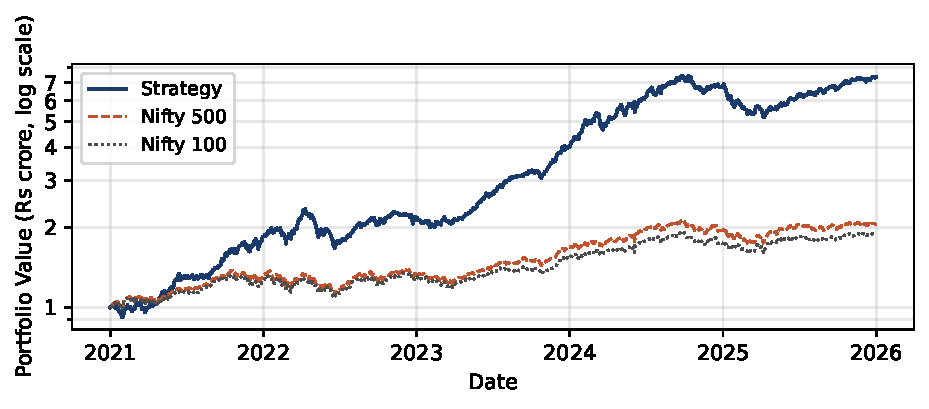
\includegraphics[width=0.72\textwidth]{equity_curve.pdf}
\caption{Portfolio value vs. Nifty 500 and Nifty 100, 2021--2025 (all series start at
Rs 1 crore).}
\end{figure}

\begin{figure}[h]
\centering
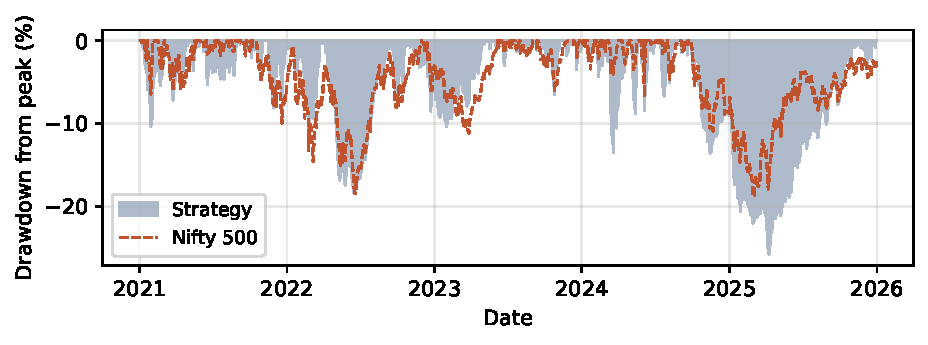
\includegraphics[width=0.72\textwidth]{drawdown.pdf}
\caption{Drawdown from running peak, strategy vs. Nifty 500, 2021--2025. The strategy's deepest
trough is the $-30.07\%$ Maximum Drawdown reported in Table 1; it subsequently recovers to a new
high.}
\end{figure}

For additional context beyond the required list, the strategy also shows Beta $\approx 1.05$ and
annualised Alpha of $+32.96\%$ against Nifty 500 (CAGR $-$ Beta $\times$ benchmark CAGR; slightly
below Table 3's raw $+33.80$pp outperformance since Beta is above 1), an Information Ratio of
2.34, a Sortino Ratio of 3.38, a Calmar Ratio of 1.63, and $R^2 \approx 0.53$ against the
benchmark.

\section{Benchmark Comparison}

\textbf{Benchmark choice.} Nifty 500 (index \texttt{\^{}CRSLDX}) is used as the primary
benchmark because the eligible universe spans large, mid and small caps. A broad,
$\approx$500-name, all-cap index is a more representative comparator than a large-cap-only index
such as Nifty 100. Nifty 100 is reported alongside for completeness.

\begin{table}[h]
\centering
\begin{tabular}{lrrr}
\toprule
& \textbf{Strategy} & \textbf{Nifty 500} & \textbf{Nifty 100} \\
\midrule
CAGR & 49.15\% & 15.36\% & 13.35\% \\
Total Return, 2021--2025 & 637.19\% & 104.17\% & 87.07\% \\
Maximum Drawdown & $-$30.07\% & $-$18.84\% & $-$17.56\% \\
Sharpe Ratio (rf = 0\%) & 2.35 & 1.07 & 0.94 \\
\bottomrule
\end{tabular}
\caption{Strategy vs. benchmark, full 2021--2025 window.}
\end{table}

The strategy outperforms both benchmarks by a wide margin on CAGR and total return, at the cost
of a somewhat deeper maximum drawdown than Nifty 500--expected for a concentrated 10-stock
book relative to a $\approx$500-name index, and discussed further below.

\begin{table}[h]
\centering
\begin{tabular}{lrrr}
\toprule
\textbf{Year} & \textbf{Strategy} & \textbf{Nifty 500} & \textbf{Nifty 100} \\
\midrule
2021 & +84.32\% & +30.19\% & +25.04\% \\
2022 & +18.31\% & +3.02\% & +3.63\% \\
2023 & +82.87\% & +25.76\% & +20.05\% \\
2024 & +68.81\% & +15.16\% & +11.76\% \\
2025 & +9.50\% & +6.69\% & +8.96\% \\
\bottomrule
\end{tabular}
\caption{Calendar-year returns, strategy vs. benchmarks. The strategy leads in every year,
including the weak-market year 2022, when both benchmarks were roughly flat.}
\end{table}

\section{Limitations and Discussion}

\textbf{Concentration and momentum-crash risk.} Holding 10 stocks concentrates idiosyncratic
risk far more than a 500-name benchmark, and a momentum tilt adds a specific failure mode on top:
trending stocks can reverse sharply once a rally becomes crowded (a ``momentum crash''). This is
not theoretical -- a two-factor version of this strategy (momentum and low-volatility only, no
quality/trend-smoothness) returned $-5.40\%$ in a blind 2025 test, while Nifty 500 returned
$+4.61\%$. Adding the quality factor fixed this in the same test ($+7.93\%$), but one held-out
year does not guarantee immunity to a different kind of reversal in the future.

\textbf{A tested and rejected risk control.} A portfolio-level drawdown circuit breaker
(de-risking 50\% of the book whenever it fell more than 8\% from its post-rebalance peak) was
tested against a 20-quarter rolling grid. It shrank the worst single quarter's excess over
benchmark from $-10.68$pp to $-9.00$pp and reduced full-period maximum drawdown from $-30.07\%$
to $-25.15\%$, and Sharpe actually improved slightly (2.35 to 2.50). However, it cut Total Net
PnL from Rs 6.37cr to Rs 5.35cr and CAGR from 49.15\% to 44.76\%. Since Total Net PnL is the
primary Round 2 ranking metric, this was a deliberate, metrics-driven decision to exclude the
breaker, not an oversight. It reflects a real trade-off between shallower drawdowns and the
metric the round is actually scored on.

\begin{figure}[h]
\centering
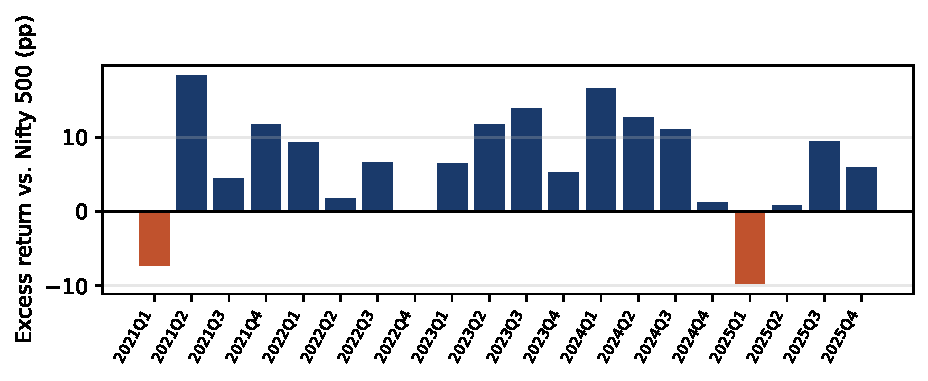
\includegraphics[width=0.72\textwidth]{quarterly_excess.pdf}
\caption{Excess return over Nifty 500 in each of the 20 independent calendar-quarter backtests
used for the robustness grid above (the submitted strategy). 16 of 20 quarters (80\%) beat the
benchmark; the four losing quarters (2021Q1, 2022Q2, 2024Q4, 2025Q1) are visible as the bars
below zero.}
\end{figure}

\textbf{Execution friction.} All sells for a rebalance execute before any buys, so freed-up
cash from trimmed or dropped positions is available to fund new and increased ones. Even so,
because the ten target weights sum to exactly 100\% of portfolio value while every buy also
carries the 0.1\% transaction cost on top, fully funding all ten names structurally needs
slightly more capital than is available; the lowest-priority name is typically left short once
whole-share flooring is applied. Rather than let that shortfall sit idle, it is redeployed into
the names that were funded (Section 3.2). Selection also does not itself check trend status, so
a name can score well on momentum/low-volatility/quality while already trading below its own
200-day average on rebalance day; such a name is simply not bought that quarter (its allocation
is zeroed), and may be selected again at a later rebalance once it recovers above its own
average. Names being trimmed this quarter are also excluded from redeployment.

\textbf{Universe timing.} Using current (rather than historical, point-in-time) index
constituent lists for the full 2021--2025 backtest is a simplification driven by data
availability; a small number of names in the backtest may not have been constituents of their
respective index for the entire period.

\textbf{No fundamental data.} The strategy is intentionally price-only. This avoids a real
data-reliability problem for small and mid caps, but it also means the model cannot see
valuation, earnings quality, or balance-sheet risk directly. It would not be expected to perform
well in a regime where price-momentum and fundamentals diverge sharply.

\end{document}
